\chapter{Architectural Overview}
\label{chapter:archoverview}

The design of ACE is split into three independent layers. 
Each layer has a well-defined interface between the adjacent layers and 
well-defined responsibilities. A layer accesses only its adjacent layers.
The layered design has several distinct advantages:

\begin{itemize} 
 \item a layer implementation could easily be replaced
 \item clear separation makes working independently much easier
 \item ACE could be used as framework for other collaborative applications, for instance a shared whiteboard
\end{itemize}


\begin{figure}[H]
 \centering
 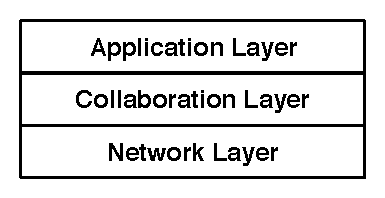
\includegraphics[width=5.96cm,height=2.79cm]{../images/finalreport/architecture_layers.eps}
 \caption{The Layers of ACE}
\end{figure}

\paragraph{Application Layer:} The application layer consists mainly in the 
graphical user interface. The layer implementation in ACE is built with
Java Swing.

\paragraph{Collaboration Layer:} The collaboration layer provides the
collaborative editing functionality to the application layer. It hosts the core
consistency control algorithm, which is based on the concept of operational 
transformation. By replacing the collaboration layer it would be theoretically 
possible to replace the employed consistency control algorithm. Further it uses 
the network layer for all network related functionality.

\paragraph{Network Layer:} The network layer is the lowest layer of ACE. It 
provides networking functionality to the collaboration layer. The two most 
important features are discovery of users and documents as well as communication 
with other users and sessions. Replacing the network layer allows to use a 
different network technology and/or a different protocol.



\section{Preliminaries}

\subsection{Identifiers}
ACE knows different types of identifiers. The algorithm works with so-called
site ids. They are used on the level of the algorithm to break priority
ties when transforming operations. As \emph{Jupiter} works only with two
sites, the site id is always either zero (server-side) or one (client-side).

Further, there is a session-wide unique identifier that uniquely identifies
a user in the session. A user in the session is called a participant, thus
this id is the participant id.

Lastly, both users and published documents have a globally unique identifer
primarily used by the network layer to identify users and documents.


\subsection{Awareness Information}
ACE supports sending updates to the text insertion caret and the selection
to the session. This information is displayed in the GUI to make users
aware of the actions of other users. The two classes \texttt{Caret\-Update}
and \texttt{Caret\-Update\-Message} are used to encapsulate that information.

A \texttt{Caret\-Update\-Message} consists of the site id of the sender, the
timestamp at the sender's site, and a \texttt{Caret\-Update} object. The
\texttt{Caret\-Update} has a \texttt{dot} and a \texttt{mark} property. The
\texttt{dot} specifies the position of the insertion point, \texttt{mark} 
specifies the end of the selection. If both \texttt{dot} and \texttt{mark} are 
equal, nothing is selected. 

\begin{figure}[H]
 \centering
 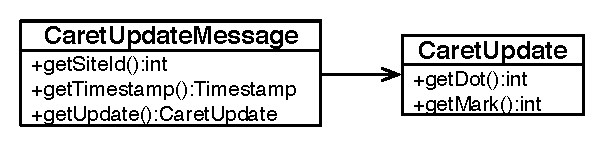
\includegraphics[width=9.7cm,height=1.9cm]{../images/finalreport/collaboration_caretupdate_uml.eps}
 \caption{CaretUpdate and CaretUpdateMessage}
\end{figure}



\section{Interface Application/Collaboration Layer}
The interfaces between the application and the collaboration layer are in
the package \texttt{ch.\-iserver.\-ace.\-collboration}. In the following,
the package name is omitted for space reasons. The main interface in
the collaboration layer is the \texttt{Collaboration\-Service}.
It is the entry point for an application layer implementation. The main 
functionality exposed by the collaboration service is:
\begin{itemize}
 \item discovery of users and documents
 \item publishing of local documents
 \item registering invitation callback for receiving invitations
 \item service failure reporting
 \item changing of local user's information
\end{itemize}


\subsection{Collaboration Service}

\begin{figure}[H]
 \centering
 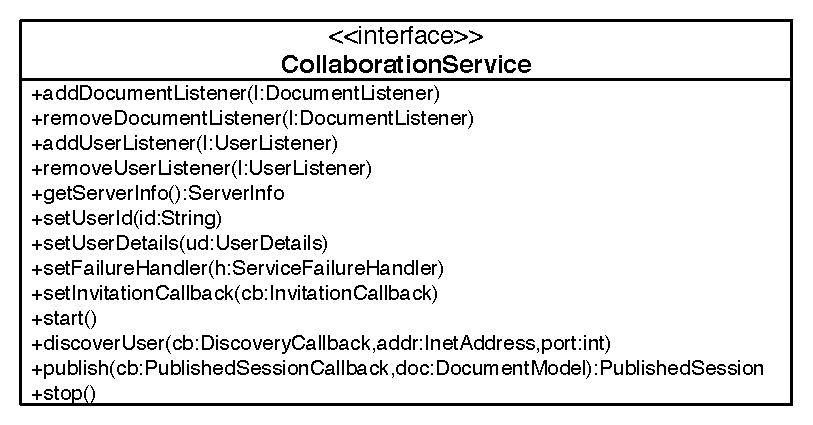
\includegraphics[width=13.19cm,height=6.63cm]{../images/finalreport/architecture_collaborationservice_uml.eps}
 \caption{CollaborationService Interface}
\end{figure}

The \texttt{Collaboration\-Service} has to be initialized before it can
be used. This includes typically the following steps:

\begin{enumerate}
 \item setting local user id
 \item setting local user details
 \item adding listeners
 \item setting callbacks
\end{enumerate}

Each running instance of ACE needs a unique user id. This id is used to uniquely
identify users. The user id is set with the \texttt{set\-User\-Id} method. The
user details (at the moment just the display name of the user) are set with
\texttt{set\-User\-Details} method.

Further, the \texttt{Collaboration\-Service} provides the possibility to set a
\texttt{Service\-Failure\-Handler} 
(see figure \ref{fig:archoverview.servicefailurehandler}). 
This failure handler is notified about 
service failures and is set with the \texttt{set\-Failure\-Handler} method. 
A typical service failure occurs if the port used by
ACE is already in use by another application. The failure handler is used
to pass service level failures to the application. Session level failures
are handled differently (see \ref{sect:archoverview.sessionfailure}). 

\begin{figure}[H]
 \centering
 
\includegraphics[width=8.08cm,height=1.52cm]{../images/finalreport/architecture_servicefailurehandler_uml.eps}
 \caption{ServiceFailureHandler Interface}
 \label{fig:archoverview.servicefailurehandler}
\end{figure}


The registration of listeners as well as the setting of the invitation 
callback are discussed in the next section.

Once all the necessary setup steps have been performed, the
\texttt{Collaboration\-Service} can be started with a call to the
\texttt{start} method. At the end of the lifecycle of the
service, the \texttt{stop} method should be called.

The \texttt{get\-Server\-Info} method can be used to get the local 
\texttt{Server\-Info} object, which specifies the IP and port of the
local server. Note that this information may not be available right
from the beginning, as it could be dynamically be determined when the
service is started. The application should therefore poll for that information
until it is available (e.g. with a timer). This situation could be improved
by use of a callback object.


\subsection{Discovery}
\label{sect:archoverview.discovery}
The collaboration service provides a listener registration mechanism for
users and documents. The corresponding methods are \texttt{add\-User\-Listener}
and \texttt{add\-Document\-Listener}. These listeners are notified whenever a
new user or document is discovered by the underlying network layer. The two 
listener interfaces are pretty similar. 

\begin{figure}[H]
 \centering
 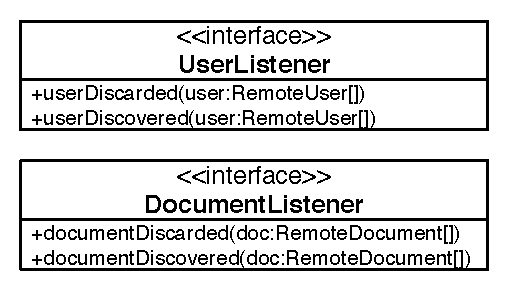
\includegraphics[width=8.04cm,height=4.34cm]{../images/finalreport/architecture_listener_uml.eps}
 \caption{DocumentListener and UserListener Interfaces}
\end{figure}

The parameters are instances of type \texttt{Remote\-User} and
\texttt{Remote\-Document} respectively. The user objects have a \texttt{name}
property and documents have a \texttt{title} property. Further, they support
property change events that are used to notify registered 
\texttt{Property\-Change\-Listener} instances about property value changes. 
The collaboration layer guarantees that for each unique user and document
there is only one \texttt{Remote\-User} and \texttt{Remote\-Document}. 
This makes
it possible to register \texttt{Property\-Change\-Listener}s to be 
notified about changes to the user name and document title. 

Both, users and documents, have a unique id. This id is mainly used by the
network layer to uniquely identify users and documents in protocol messages.

\begin{figure}[H]
 \centering
 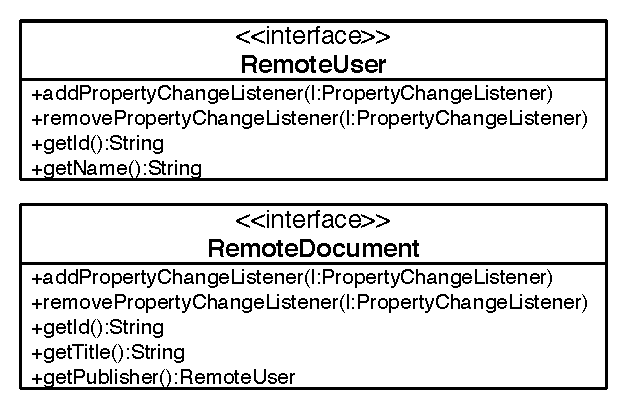
\includegraphics[width=10.05cm,height=6.35cm]{../images/finalreport/architecture_userdocument_uml.eps}
 \caption{RemoteUser and RemoteDocument Interface}
\end{figure}

The \texttt{Remote\-Document} objects have also a property of type
\texttt{Remote\-User} for the publisher of the document.


\subsection{Explicit User Discovery}
The described discovery mechanism relies on the services of the network layer.
It usually relies on IP multicast, which is most likely not available outside
of the local subnet. ACE therefore provides an explicit way to discover users.
The \texttt{Collaboration\-Service} has a method \texttt{discover\-User} with
three parameters: a \texttt{Discovery\-Callback} to report the result
of the discovery, an \texttt{Inet\-Address} specifying the host, and a port.

\begin{figure}[H]
 \centering
 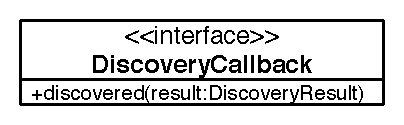
\includegraphics[width=6.28cm,height=1.55cm]{../images/finalreport/architecture_discoverycallback_uml.eps}
 \caption{DiscoveryCallback Interface}
\end{figure}

The callback is notified about the result of the discovery. The passed in
\texttt{Discovery\-Result} has a status and a status message. If the status
is equal to \texttt{Discovery\-Result.\-SUCCESS} the discovery succeeded. The
discovered user is returned through the normal code path, i.e. the
registered \texttt{User\-Listener} objects receive a notification. (see
section \ref{sect:archoverview.discovery})

\begin{figure}[H]
 \centering
 
\includegraphics[width=4.94cm,height=1.91cm]{../images/finalreport/architecture_discoveryresult_uml.eps}
 \caption{DiscoveryResult}
\end{figure}


\subsection{Joining Documents}
\label{sect:archoverview.join}
\texttt{Remote\-Document} instances have a \texttt{join} method. It
can be used to join a published document. All that is needed to
join a document is to register a \texttt{Document\-Listener} with the 
\texttt{Collaboration\-Service} and call \texttt{join} on a discovered document.

The \texttt{join} method is designed to return immediately. Join is a 
potentially long running operation. First, the join request has to be sent
to the publisher. Second, it might take some time to transfer the document
content over the network. And last but not least, joining might need the 
approval of the publisher, which might take even longer. Thus, it is a 
necessary design decision to make this method asynchronous.

The result of join request is communicated to an object passed to the
\texttt{join} method implementing the \texttt{Join\-Callback} interface.

\begin{figure}[H]
 \centering
 
\includegraphics[width=8.43cm,height=1.94cm]{../images/finalreport/architecture_joincallback_uml.eps}
 \caption{JoinCallback Interface}
\end{figure}

Depending on the outcome of the join request, either \texttt{accepted} or
\texttt{rejected} is called. The \texttt{accepted} method takes an argument
of type \texttt{Session} and returns a \texttt{Participant\-Session\-Callback}. 
The session
is the object that represents a collaborative editing session. It is
implemented by the collaboration layer and passed to the application layer.
The \texttt{Participant\-Session\-Callback} in turn is returned by the 
application layer to the collaboration layer and is used by it to return 
received operations and caret updates from other participants in the session.


\subsection{Publishing Documents}
To publish a document, the \texttt{Collaboration\-Service} \texttt{publish}
method is used. The method has two parameters. The first is the session callback
for a published session (\texttt{Published\-Session\-Callback}). 
The second method is the \texttt{Document\-Model}
of the document to be published. The \texttt{Document\-Model} contains the
document content, the title, as well as the current caret position of the
publisher. The collaboration service in turn returns an object of type
\texttt{Published\-Session}, which is used both to control the session as well
as sending operations and updates of the caret position.


\subsection{Inviting Users}
\label{sect:archoverview.invitingusers}
The \texttt{Published\-Session} has a method \texttt{invite} to invite users.
The invite method has as single parameter of type \texttt{Remote\-User}. 
The invite method is non-blocking, i.e. it
returns immediately. If the user accepts the invitation, he is added to the
list of participants of the session. The API does not provide a way to return
a feedback to the application layer whether the invitation is accepted.
Future versions may improve in that area and add a callback interface 
to notify the publisher about the action taken on the invitation.


\subsection{Receiving Invitations}
\label{sect:archoverview.invitation}
The \texttt{CollaborationService} has a method to register an
\texttt{InvitationCallback}. This callback is notified whenever another user
tries to invite the local user. 

\begin{figure}[H]
 \centering
 
\includegraphics[width=6.84cm,height=1.52cm]{../images/finalreport/architecture_invitationcallback_uml.eps}
 \caption{InvitationCallback Interface}
\end{figure}

The passed in \texttt{Invitation} allows to retrieve the document for which
the user is invited as well as inviter. The
methods are \texttt{accept} and \texttt{reject}. They represent
the user actions of accepting or rejecting an invitation. 

\begin{figure}[H]
 \centering
 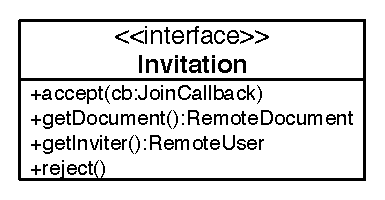
\includegraphics[width=5.96cm,height=2.82cm]{../images/finalreport/architecture_invitation_uml.eps}
 \caption{Invitation Interface}
\end{figure}

The \texttt{accept} method has as parameter a \texttt{Join\-Callback}. This
callback is used exactly in the same way as the \texttt{Join\-Callback} passed
to the \texttt{join} method of the \texttt{Remote\-Document} 
(see \ref{sect:archoverview.join}).


\subsection{Communicating with a Session}
Until now, we have not discussed how to communicate with a session. An
editing session is represented by the \texttt{Session} interface.
We have shown several ways to get a \texttt{Session} object:

\begin{itemize}
 \item joining a discovered remote document
 \item accepting an invitation
 \item publishing a local document (\texttt{PublishedSession})
\end{itemize}

All those ways have one thing in common: the application layer has to pass a 
\texttt{Session\-Callback}
(in case of publish a \texttt{Published\-Session\-Callback} and in every
other case a \texttt{Participant\-Session\-Callback}) to the collaboration
layer. There are always these two objects, a \texttt{Session} and
a \texttt{Session\-Callback}. The \texttt{Session} is used by the application
layer to send events to the collaboration layer and a \texttt{Session\-Callback}
is used to notify the application layer about session related events from the 
collaboration layer. Figure \ref{fig:archoverview.sessionandcallback} depicts 
this situation.

\begin{figure}[H]
 \centering
 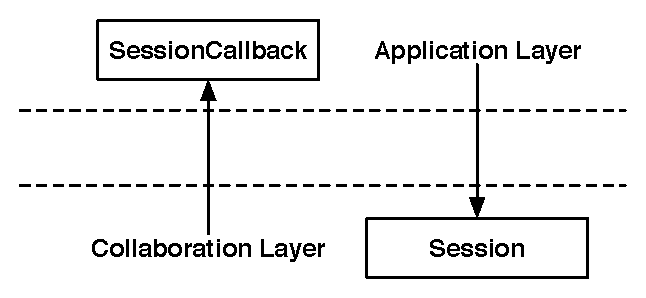
\includegraphics[width=10.37cm,height=4.48cm]{../images/finalreport/architecture_session_sessioncallback.eps}
 \caption{Session and SessionCallback}
 \label{fig:archoverview.sessionandcallback}
\end{figure}

The figure \ref{fig:archoverview.session} shows the \texttt{Session} interface
hierarchy.

\begin{figure}[H]
 \centering
 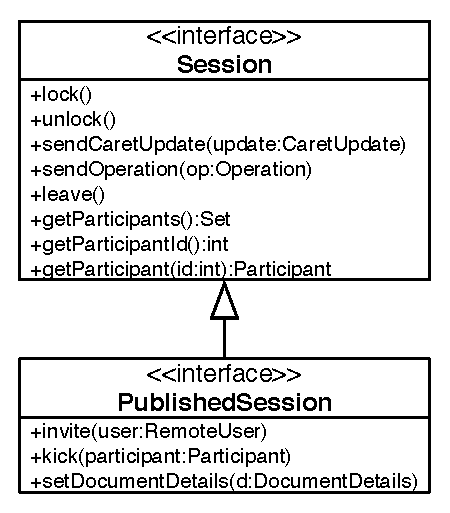
\includegraphics[width=7.06cm,height=8.11cm]{../images/finalreport/architecture_session_uml.eps}
 \caption{Session and PublishedSession Interface}
 \label{fig:archoverview.session}
\end{figure}


\subsubsection{Locking}
In order that the system can guarantee the consistency of the replicas, we
must employ a locking scheme in the session and the document model of
the application layer implementation. The locking has to ensure that:

\begin{itemize}
 \item the local document does not change while a remote request is 
transformed
 \item the local document does not change while generating a local request (as a result of the user typing text)
\end{itemize}

Before determining the index and the text of a local operation, the session must
be locked. This ensures that from the point where the operation's parameters
are determined
to the point where a request is created for the operation the document does
not change. Failing to properly lock would potentially result in an invalid index of the local operation, because a processed remote operation could 
shift the text.

The \texttt{Session\-Callback} has a method \texttt{get\-Lock}, from which
the collaboration layer gets a lock from the application layer. This
lock is used inside the session as well as it is available through the
\texttt{lock} and \texttt{unlock} methods of the \texttt{Session} interface.
Make sure that for each call to
\texttt{lock} there is a matching \texttt{unlock} call. To be sure that unlock
is called, it must be placed inside a finally block.

\begin{figure}[H]
 \small{\begin{verbatim}
    Session session = ...;
    session.lock();
    try {
      Operation op = ...;
      session.sendOperation(op);
    } finally {
      session.unlock();
    }
 \end{verbatim}}
 \caption{Proper locking of a Session}
\end{figure}

The documentation of the application layer (see chapter 
\ref{chapter:applicationlayer}) 
shows how the lock is implemented in our application layer implementation.


\subsubsection{Sending Operations}
The \texttt{send\-Operation} and \texttt{send\-Caret\-Update} 
methods are used to send locally generated operations or
caret updates to the other participants in the session. 

\subsubsection{Leaving the Session}
The \texttt{leave} method allows to leave the session, i.e. stop participating. 

\subsubsection{Participant related methods}
The participant
related methods allow to access the currently participating users. These
methods return objects implementing the \texttt{Participant} interface. This
interface has two methods, one to get the \texttt{Remote\-User} and one to get 
the participant id.

\begin{figure}[H]
 \centering
 
\includegraphics[width=4.34cm,height=1.98cm]{../images/finalreport/architecture_participant_uml.eps}
 \caption{Participant Interface}
\end{figure}

A participant id is a session-wide unique identifier for a user. They are given
to a user when he joins a session by the publisher of the session. The local
participant id can be retrieved by the \texttt{get\-Participant\-Id} method.


\subsubsection{PublishedSession}
The \texttt{Published\-Session} has some additional methods that correspond
to the additional actions available to the publisher of a document. The
publisher can change the name of the document through the
\texttt{set\-Document\-Details} method. This can be used by the application
to change the title when the document is saved as a different file.
The \texttt{invite} method we have already seen in action in the section
\ref{sect:archoverview.invitingusers}.

Last but not least, the \texttt{kick} method can be used to kick a
participant from the session. This gives the publisher the power to
ban a misbehaving user from the session.


\subsection{Session Callbacks}
\begin{figure}[H]
 \centering
 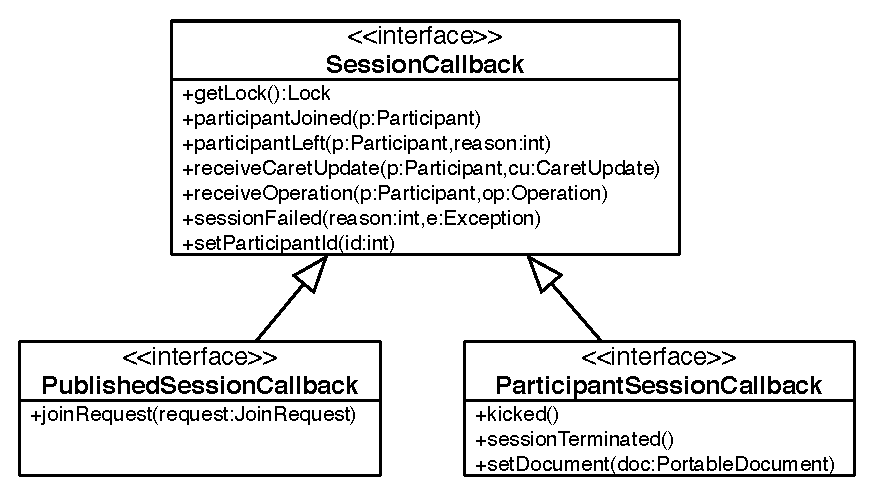
\includegraphics[width=14.25cm,height=7.83cm]{../images/finalreport/architecture_sessioncallback_uml.eps}
 \caption{SessionCallback Interfaces}
 \label{fig:archoverview.sessioncallback}
\end{figure}

The \texttt{Session\-Callback} contains the methods common to the callbacks for 
both session types: the participant and the publisher session. The 
\texttt{Participant\-Session\-Callback} adds methods that are only meaningful 
for participants and the \texttt{Published\-Session\-Callback} adds meaningful
for the publisher.


\subsubsection{Initialization and Termination of Participant Sessions}
When joining a document or accepting an invitation the session is passed to
the \texttt{Join\-Callback}'s \texttt{accepted} method. This method has a
parameter of type \texttt{Participant\-Session\-Callback}. The first two
methods called on that callback object are \texttt{set\-Participant\-Id}, which 
communicates the assigned participant id of the local participant, and 
\texttt{set\-Document}, which sets the document. After these methods are called
all the other methods can be called by the session.

The \texttt{set\-Document} method gets a \texttt{Portable\-Document} instance
as parameter. It represents the document content at join time. A portable
document consists of a set of participants, their selections, as well as
a collection of fragments. A fragment is simply a continous run of text
created by one particular participant.

\begin{figure}[H]
 \centering
 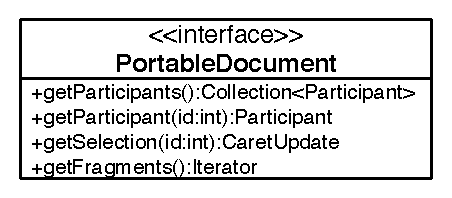
\includegraphics[width=7.09cm,height=2.79cm]{../images/finalreport/architecture_portabledocument_uml.eps}
 \caption{PortableDocument Interface}
\end{figure}

The \texttt{kicked} method is called when the local participant
has been kicked from the session. The \texttt{sessionTerminated}
method is called when the publisher conceals the published document. 

Additionally a session can fail. Session failures are common to publisher
sessions too and are described in the next section.


\subsubsection{Session Failures}
\label{sect:archoverview.sessionfailure}
The \texttt{sessionFailed}
method is used by the collaboration layer to notify the application layer
about a failed session. Reasons for this include failing network connection
to the publisher or unrecoverable situations in the collaboration or network
layer. The session should no longer be used after this method has been
called.


\subsubsection{Reception}
The callback has methods to notify the client of the session about caret
updates and operations from other participants in the session. These methods
are named \texttt{receive\-Operation} and \texttt{receive\-Caret\-Update}
and accept both a \texttt{Participant} object (the creator of the operation
or caret update)
as well as either an \texttt{Operation} or a \texttt{Caret\-Update}.


\subsubsection{Participation Events}
The \texttt{participant\-Joined} and \texttt{participant\-Left} methods
are used to notify the callback about
participants that joined or left the session. The initial set of participants
can be retrieved from the session when the document is set with
the \texttt{get\-Participants} method.


\subsubsection{PublishedSessionCallback}
The \texttt{Published\-Session\-Callback} method has a single additional method
\texttt{join\-Request} which has a parameter of type \texttt{Join\-Request}. It
is invoked whenever a user tries to join the session. The publisher of the
session can then decide if the user is allowed to join. 
The \texttt{Join\-Request}
has a single property named \texttt{user} of type \texttt{Remote\-User}, 
which is the user that 
tries to join. The request can either be accepted or rejected with the 
corresponding methods \texttt{accept} or \texttt{reject}.

\begin{figure}[H]
 \centering
 
\includegraphics[width=4.34cm,height=2.40cm]{../images/finalreport/architecture_joinrequest_uml.eps}
 \caption{JoinRequest Interfaces}
\end{figure}



\section{Interface Collaboration/Network Layer}
In the last section we had a look at the interface between the application and
the collaboration layer. The collaboration layer itself cannot implement a
collaborative editor by itself. It needs a layer that provides the networking
functionality, the network layer. The network layer should not be used
directly by the application layer. The interfaces described in this 
section can all be found in the \texttt{ch.\-iserver.\-ace.\-net} package.


\subsection{Network Service}
The \texttt{Network\-Service} interface is the entry point into the network 
layer. Its functionality and responsibilities are in some aspects similar to the 
\texttt{Collaboration\-Service} in the collaboration layer. 

\begin{figure}[H]
 \centering
 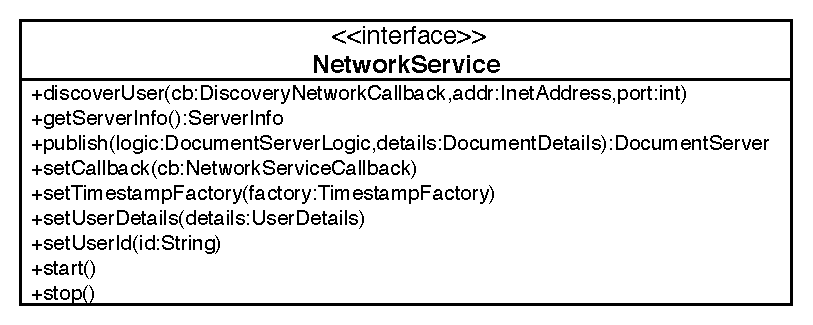
\includegraphics[width=13.19cm,height=4.94cm]{../images/finalreport/architecture_networkservice_uml.eps}
 \caption{NetworkService Interface}
 \label{fig:archoverview.networkservice}
\end{figure}

Before the \texttt{Network\-Service} can be used, the following steps have
to be done:

\begin{enumerate}
 \item setting local user id (\texttt{set\-User\-Id})
 \item setting local user details (\texttt{set\-User\-Details})
 \item setting the timestamp factory (\texttt{set\-Timestamp\-Factory})
 \item setting the network service callback (\texttt{set\-Callback})
\end{enumerate}

Then, the \texttt{start} method must be called. At the end of the lifecycle
of the service, the \texttt{stop} method should be called to properly shutdown
the service. Calling any method after the call to \texttt{stop} should
throw an \texttt{Illegal\-State\-Exception}.


\subsection{TimestampFactory}
The collaboration layer has to set a \texttt{Timestamp\-Factory} on the
\texttt{NetworkService} with the \texttt{set\-Timestamp\-Factory} method. This
factory is used to convert a timestamp from a generic format (an array of
integers) into a \texttt{Timestamp} object which can be understood by the
collaboration layer. The \texttt{Timestamp} interface has a method which 
achieves the inverse operation, it is called \texttt{get\-Components} and
returns an integer array.

\begin{figure}[H]
 \centering
 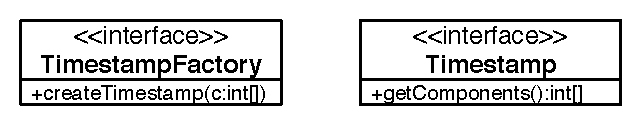
\includegraphics[width=10.30cm,height=1.55cm]{../images/finalreport/architecture_timestampfactory_uml.eps}
 \caption{TimestampFactory and Timestamp Interface}
\end{figure}


\subsection{Network Service Callback}
The \texttt{Network\-Service} interface has a method 
\texttt{set\-Network\-Service\-Callback}. The network layer provides a tighter
one-to-one binding between itself and the upper layer through this
callback interface. Instead of exposing a set of listeners
(such as those provided by the collaboration layer: \texttt{User\-Listener}
and \texttt{Document\-Listener}), it provides one unified callback interface.

\begin{figure}[H]
 \centering
 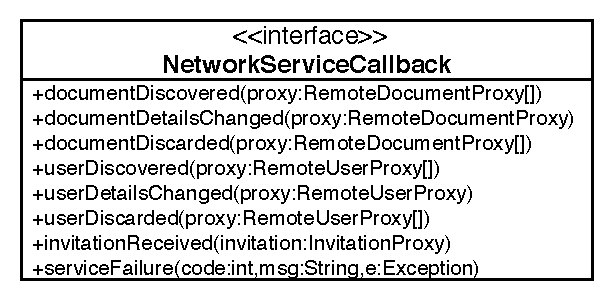
\includegraphics[width=9.81cm,height=4.52cm]{../images/finalreport/architecture_networkservicecallback_uml.eps}
 \caption{NetworkServiceCallback Interface}
\end{figure}


\subsubsection{Discovery}
\label{sect:archoverview.net.discovery}
The discovery results for documents are communicated through the 
\texttt{document\-Discovered}, \texttt{document\-Discarded}, and the
\texttt{document\-Details\-Changed} methods. Similar methods exist for user
discovery (\texttt{user\-Discovered}, \texttt{user\-Details\-Changed}, 
\texttt{user\-Discarded}). These methods are similar to the 
\texttt{User\-Listener} and \texttt{Document\-Listener} methods except that they
pass \texttt{Remote\-User\-Proxy} as well as \texttt{Remote\-Document\-Proxy} 
objects. Additionally, there are the two methods 
\texttt{document\-Details\-Changed}
and \texttt{user\-Details\-Changed}. These are called whenever the details of
a document or user changed. This is in contrast to the collaboration layer,
where these change events are passed as \texttt{Property\-Change\-Event}s to
registered \texttt{Property\-Change\-Listener}s.

\begin{figure}[H]
 \centering
 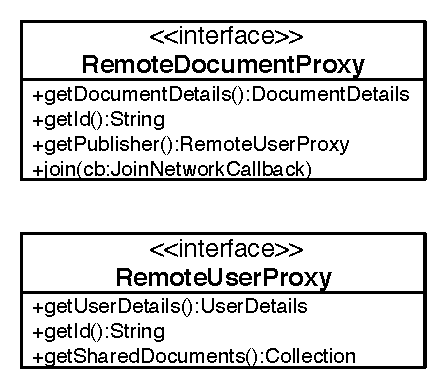
\includegraphics[width=6.99cm,height=6.00cm]{../images/finalreport/architecture_userdocumentproxy_uml.eps}
 \caption{RemoteDocumentProxy and RemoteUserProxy Interfaces}
 \label{fig:archoverview.userdocumentproxy}
\end{figure}


\subsubsection{Receiving Invitations}
The network layer passes received invitations to the 
\texttt{Network\-Service\-Callback}'s \texttt{invitation\-Received} method.
This method has a parameter of type \texttt{Invitation\-Proxy}, which 
corresponds to the \texttt{Invitation} object in the collaboration layer.
(see section \ref{sect:archoverview.invitation}).

\begin{figure}[H]
 \centering
 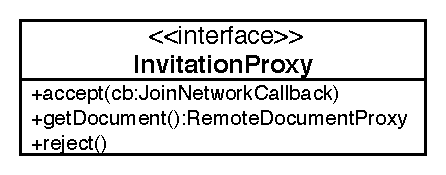
\includegraphics[width=6.99cm,height=2.40cm]{../images/finalreport/architecture_invitationproxy_uml.eps}
 \caption{InvitationProxy Interface}
\end{figure}

The invitation can be either be accepted or rejected with the methods
\texttt{accept} or \texttt{reject} respectively. The document for which
the invitation is meant is accessible throught the \texttt{get\-Document}
method.


\subsubsection{Service Failures}
Service failures are passed to the \texttt{Network\-Service\-Callback} through
the \texttt{service\-Failure} method.


\subsection{Explicit User Discovery}
The method \texttt{discover\-User} in the \texttt{Network\-Service} is used to 
start an explicit discovery
of another user, for instance over the Internet. It corresponds to the
\texttt{discover\-User} method in the \texttt{Collaboration\-Service}. The
only difference is, that it accepts a \texttt{Discovery\-Network\-Callback}
instance (instead of a \texttt{Discovery\-Callback} instance). The result
of the discovery is communicated through the methods 
\texttt{user\-Discovery\-Failed} and \texttt{user\-Discovery\-Succeeded} method.
The actual discovered user (if the discovery is successful) is passed 
through the \texttt{Network\-Service\-Callback}'s \texttt{user\-Discovered} 
method.

\begin{figure}[H]
 \centering
 
\includegraphics[width=7.62cm,height=1.98cm]{../images/finalreport/architecture_discoverynetworkcallback_uml.eps}
 \caption{DiscoveryNetworkCallback Interface}
\end{figure}


\subsection{Joining Documents}
Documents are discovered through the \texttt{Network\-Service\-Callback} methods
described above (see section \ref{sect:archoverview.net.discovery}). A discovered document is represented by a \texttt{Remote\-Document\-Proxy} instance (see figure \ref{fig:archoverview.userdocumentproxy}). 
This object provides similar methods
to the ones in the \texttt{Remote\-Document} interface. The \texttt{join}
method allows to join the given document. The only parameter to that method
is an implementation of the \texttt{Join\-Network\-Callback} interface.

\begin{figure}[H]
 \centering
 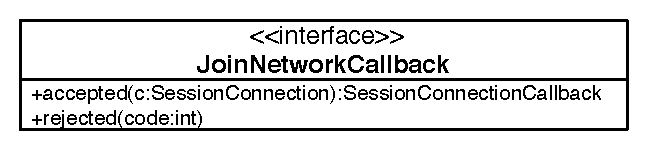
\includegraphics[width=10.41cm,height=1.98cm]{../images/finalreport/architecture_joinnetworkcallback_uml.eps}
 \caption{JoinNetworkCallback Interface}
\end{figure}

This interface has two methods, \texttt{accepted} and \texttt{rejected}.
The \texttt{rejected} method notifies the callback that the join
was rejected. The passed in \texttt{code} argument specifies the reason, why
the join was rejected. The corresponding constants are defined in the
\texttt{Join\-Request} interface (which is part of the collaboration package). 
A join can be rejected for several reasons.
To name a few: publisher rejects join, joining user is on the session's 
black list, the joining user is already in the session, etc.

On the other hand, the \texttt{accepted} method is invoked when the join
was accepted. The parameter of type \texttt{Session\-Connection} represents
the connection to the session. Its purpose corresponds to the \texttt{Session}
interface in the collaboration layer. The callback has to return a
\texttt{Session\-Connection\-Callback} implementation (whose purpose corresponds
to the \texttt{Session\-Callback} in the collaboration layer).



\subsection{Network Layer on the Participant's Side}
The participant side and the publisher side of the network layer differ
significantly.

\subsubsection{SessionConnection}
The \texttt{Session\-Connection} allows the collaboration layer to
communicate with the session. For each editing session there is
exactly one \texttt{Session\-Connection} (per participant) with its corresponding \texttt{Session\-Connection\-Callback} instance.

\begin{figure}[H]
 \centering
 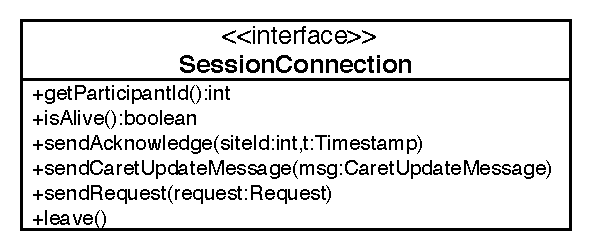
\includegraphics[width=9.45cm,height=3.67cm]{../images/finalreport/architecture_sessionconnection_uml.eps}
 \caption{SessionConnection Interface}
\end{figure}

The send methods allow the participant to send requests, caret updates,
and acknowledge messages to the session. In contrast to the session
layer the send methods deal with \texttt{Request}s (instead of
\texttt{Operation}s) and \texttt{Caret\-Update\-Message}s (instead of
\texttt{Caret\-Update}s). The
\texttt{leave} method notifies the session that the local user does
no longer want to be part of the session. The \texttt{get\-Participant\-Id}
method gives access to the assigend participant id.


\subsubsection{SessionConnectionCallback}
The \texttt{Session\-Connection\-Callback} is used by the network layer
to pass session related events to the collaboration layer.

\begin{figure}[H]
 \centering
 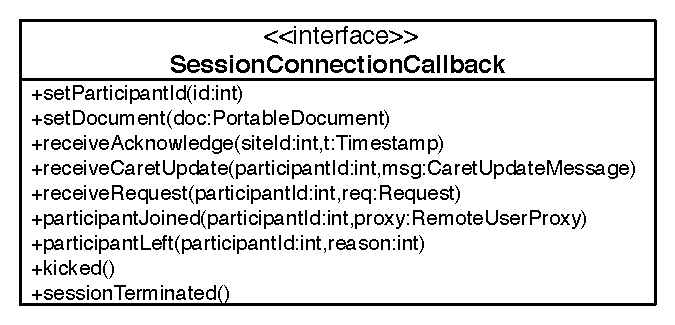
\includegraphics[width=10.87cm,height=4.94cm]{../images/finalreport/architecture_sessionconnectioncallback_uml.eps}
 \caption{SessionConnectionCallback Interface}
\end{figure}

The \texttt{receive} methods pass a received message to the collaboration
layer. The \texttt{participant\-Joined} and \texttt{participant\-Left} methods
notify the collaboration layer about changes in the set of participants.
At the beginning of the lifecycle of the session, both the participant
id and the document are passed to the callback. The document is of
type \texttt{ch.\-iserver.\-ace.\-net.\-PortableDocument}, which should not
be confused with the interface with the same name in the collaboration
layer.

\begin{figure}[H]
 \centering
 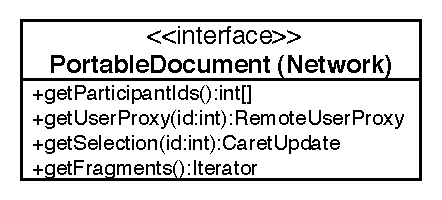
\includegraphics[width=6.91cm,height=2.82cm]{../images/finalreport/architecture_portabledocumentnet_uml.eps}
 \caption{PortableDocument Interface}
\end{figure}

The \texttt{session\-Terminated} message notifies the callback that the 
session has been closed
by the publisher of the document. The \texttt{kicked} method notifies the
callback that he has been kicked from the session.


\subsection{Network Layer on the Publisher's Side}
On the side of the publisher, the network service looks a bit different.
Let us start with explaining how a document can be published.

\subsubsection{Publishing Documents}
A document can be published through the \texttt{publish} method of the
\texttt{Network\-Service}. This method takes two arguments, one is the
\texttt{Document\-Server\-Logic} and the other is a \texttt{Document\-Details},
describing the document. The method returns a \texttt{Document\-Server}
object. These two objects are both defined as part of the interface between the
collaboration and the network layer.

\subsubsection{DocumentServer}
The \texttt{Document\-Server} interface implemented by the network layer
represents a published document to the collaboration layer. The
\texttt{invite} method will be discussed later 
(see section \ref{archoverview.net.invite}). The \texttt{set\-Document\-Details}
method allows to change the document details (currently only the title).
This method corresponds to the \texttt{set\-Document\-Details} method in
the \texttt{Published\-Session} interface of the collaboration layer.
It sends the changed document title to the other peers.

\begin{figure}[H]
 \centering
 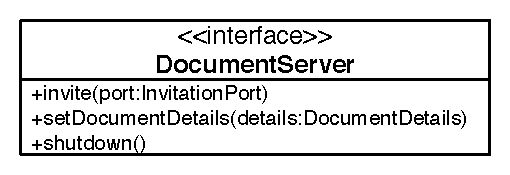
\includegraphics[width=8.08cm,height=2.40cm]{../images/finalreport/architecture_documentserver_uml.eps}
 \caption{DocumentServer Interface}
\end{figure}

Finally, the \texttt{shutdown} method is called to shutdown the document
server for the document. This should be called when a published document
is concealed.

\subsubsection{DocumentServerLogic}
\label{sect:archoverview.net.documentserverlogic}
The \texttt{Document\-Server\-Logic} represents the view of the network layer
on the collaboration layer for a published document. The only method
exposed by this interface is the \texttt{join} method, which has a single
parameter of type \texttt{Participant\-Connection}.

\begin{figure}[H]
 \centering
 
\includegraphics[width=6.99cm,height=1.55cm]{../images/finalreport/architecture_documentserverlogic_uml.eps}
 \caption{DocumentServerLogic Interface}
\end{figure}

\subsubsection{ParticipantConnection}
The \texttt{Participant\-Connection} interface provides the collaboration layer
a way to send events to a particular participant. When the \texttt{join}
method on the \texttt{Document\-Server\-Logic} returns, the network layer does
not have any way to send events to the server from the participant. That
is because the join request is not yet accepted. The result of the join
request is directly communicated to the \texttt{Participant\-Connection}.
The \texttt{get\-User} method allows the collaboration layer to extract the
user that wants to join the session.

\begin{figure}[H]
 \centering
 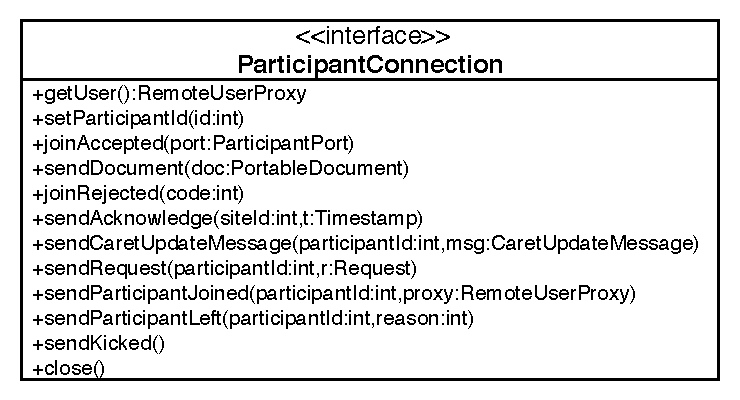
\includegraphics[width=11.96cm,height=6.21cm]{../images/finalreport/architecture_participantconnection_uml.eps}
 \caption{ParticipantConnection Interface}
\end{figure}

The \texttt{join\-Rejected} method signals that the join has been rejected. 
The passed in code specifies the reason why the join has been rejected 
(see the constants defined in the \texttt{Join\-Request} interface).
The connection is then no longer used by the collaboration layer and can thus
be destroyed.

If the join request is accepted, the following methods are called in order:
\begin{enumerate}
 \item \texttt{setParticipantId} - sets the assigend participant id for that participant
 \item \texttt{joinAccepted} - passing in an instance of the \texttt{ParticipantPort} interface
 \item \texttt{sendDocument} - sends the initial document
\end{enumerate} 

As long as the participant is part of the session, the following methods
are called:
\begin{itemize}
 \item \texttt{sendAcknowledge} 
 \item \texttt{sendCaretUpdateMessage}
 \item \texttt{sendRequest}
 \item \texttt{sendParticipantJoined}
 \item \texttt{sendParticipantLeft}
\end{itemize}

These are the basic messages sent as part of a session from the server.

The connection can be closed by a call to the \texttt{close} method. If a 
participant is kicked, first the \texttt{send\-Kicked} method and then the
\texttt{close} method is called.


\subsubsection{ParticipantPort}
The network layer gets a \texttt{Participant\-Port} implementation through
the \texttt{join\-Accepted} method. Most importantly, it has methods to receive
requests, caret update messages, as well as acknowledgements from the 
participant.

\begin{figure}[H]
 \centering
 
\includegraphics[width=8.50cm,height=3.25cm]{../images/finalreport/architecture_participantport_uml.eps}
 \caption{ParticipantPort Interface}
 \label{fig:archoverview.participantport}
\end{figure}

The \texttt{leave} method allows a participant to leave the session and
the \texttt{get\-Participant\-Id} provides a way to query the assigned
participant id.


\subsubsection{Invitations}
\label{archoverview.net.invite}
The \texttt{Document\-Server} has a method named \texttt{invite}. This method
is used by the publisher's collaboration layer to send an invitation for the
document represented by the \texttt{Document\-Server} instance. The single
argument of that method is of type \texttt{Invitation\-Port}.

\begin{figure}[H]
 \centering
 
\includegraphics[width=7.37cm,height=2.54cm]{../images/finalreport/architecture_invitationport_uml.eps}
 \caption{InvitationPort Interface}
\end{figure}

The \texttt{Invitation\-Port} provides the network layer a way to accept or
reject an invitation. The invitation is sent to the invited user. The response
of that particular user is then reported back through the 
\texttt{Invitation\-Port} to the collaboration layer of the publisher. The
method \texttt{accept} behaves similarly to the \texttt{join} method of
the \texttt{Document\-Server\-Logic} interface. The port for the accepted 
connection is passed to the \texttt{join\-Accepted} method of the passed
in connection.



\section{Fitting the Layers Together}
In the previous two sections we have discussed the two APIs between adjacent
layers separately. In this section we show how the whole fits together.
The design is based on 
interfaces. So it is impossible to say how exactly the implementation works. 
The figures represent conceptually how the layers fit together. 


\subsection{Explanations}
In figure \ref{fig:archoverview.flow.skeleton} the basic skeleton of the
figures used in the following sections is depicted. The figure shows the
three layers of ACE: application, collaboration, and network layer. In 
the following figures, these three layers are always visible. Class names
printed inside a layer (i.e. inside an area separated by dashed lines)
belong to that layer. Messages sent back and forth are shown with arrows. The
arrows have labels that correspond to the method beeing called on the target
object.

\begin{figure}[H]
 \centering
 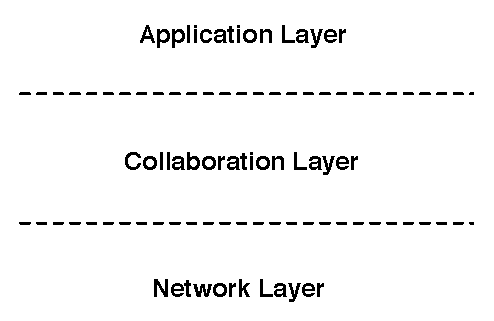
\includegraphics[width=7.80cm,height=4.87cm]{../images/finalreport/architecture_flows/skeleton.eps}
 \caption{Skeleton of Message Flows}
 \label{fig:archoverview.flow.skeleton}
\end{figure}


\subsection{Publishing a Document}
The figure \ref{fig:archoverview.flow.publish} shows how a document 
is published.
First, the \texttt{publish} method of the \texttt{Collaboration\-Service} is 
called. The collabation layer in turn calls \texttt{publish} on the
\texttt{Network\-Service}. However, the call is not simply passed through the
collaboration layer. The collaboration layer creates an object implementing
the \texttt{Document\-Server\-Logic}, which handles all the server logic of a
published document. This server logic hosts the server part of the
operational transformation algorithm. It receives requests from users, 
transforms them and forwards them to all other participants in the session.
The \texttt{Document\-Server\-Logic} represents the interface seen by the
network layer for a published document. For a description of that interface 
see section \ref{sect:archoverview.net.documentserverlogic}.

\begin{figure}[H]
 \centering
 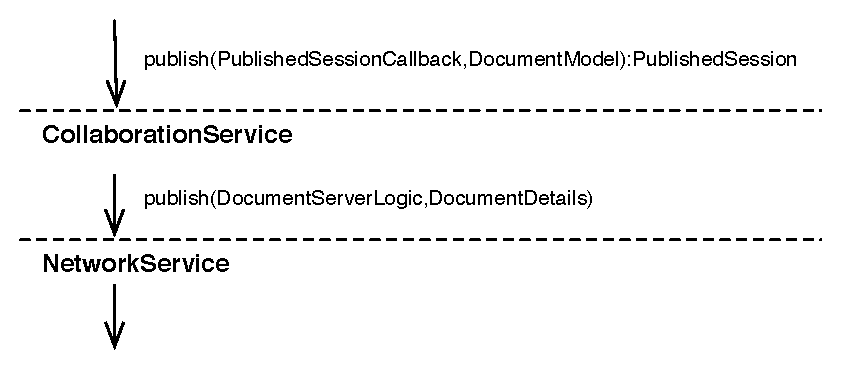
\includegraphics[width=13.69cm,height=5.72cm]{../images/finalreport/architecture_flows/publish.eps}
 \caption{Publishing a document}
 \label{fig:archoverview.flow.publish}
\end{figure}


\subsection{Discovery of Documents}
\label{sect:archoverview.flow.discovery}
A document published by one user is discovered by the other users. These
clients get notified about discovered documents through the method calls
depicted in figure \ref{fig:archoverview.flow.discovery}.

\begin{figure}[H]
 \centering
 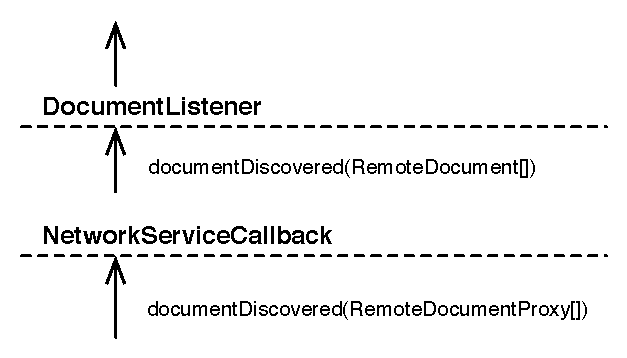
\includegraphics[width=10.05cm,height=5.50cm]{../images/finalreport/architecture_flows/discovery.eps}
 \caption{Discovery of published documents}
 \label{fig:archoverview.flow.discovery}
\end{figure}

The network layer passes discovery events to the 
\texttt{Network\-Service\-Callback}. That callback object is then responsible
to notify all registered \texttt{Document\-Listener}s. The callback receives
objects of type \texttt{Remote\-Documen\-tProxy}. It passes objects of type
\texttt{Remote\-Document} to the \texttt{Document\-Listener}s. The reason
for that separation into \texttt{Remote\-Document} and 
\texttt{Remote\-Document\-Proxy} is caused by the join procedure, which is
discussed next.


\subsection{Joining}
Joining a document consists of the following four steps:
\begin{enumerate}
 \item initiatiating join on a discovered document
 \item receiving join request by publisher
 \item accepting join request by publisher
 \item receiving join callback
\end{enumerate}

\subsubsection{Initiate Join}
\label{sect:archoverview.flow.initiatejoin}
Once a user has hold of a \texttt{Remote\-Document} he can opt to join the
published document represented by that \texttt{Remote\-Document}. In figure
\ref{fig:archoverview.flow.joininitiate} the initiating of a join
is depicted.

\begin{figure}[H]
 \centering
 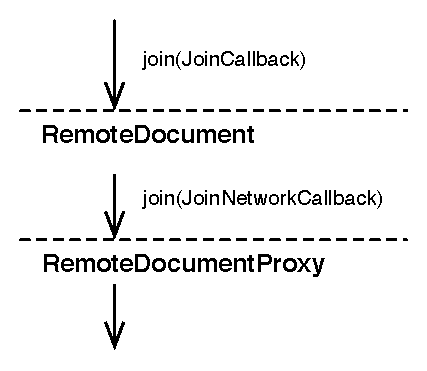
\includegraphics[width=6.67cm,height=5.72cm]{../images/finalreport/architecture_flows/join_initiate.eps}
 \caption{Initiate a join request on the joiners site}
 \label{fig:archoverview.flow.joininitiate}
\end{figure}

The \texttt{join} method on the \texttt{Remote\-Document} takes an object of
type \texttt{Join\-Callback}. This callback is used later to notify the
user that tries to join about the outcome of the join request (accepted or
rejected). The \texttt{join} method on the \texttt{Remote\-Document\-Proxy} has
a single parameter of type \texttt{Join\-Network\-Callback}. The separation
into two different callback interfaces is caused by the fact that the
collaboration layer needs to add some processing when the join callback
is invoked.

\subsubsection{Receive Join Request}
The publisher of a document is notified about a user that wants to join. 
This happens through the method calls depicted in figure 
\ref{fig:archoverview.flow.joinrequest}.

\begin{figure}[H]
 \centering
 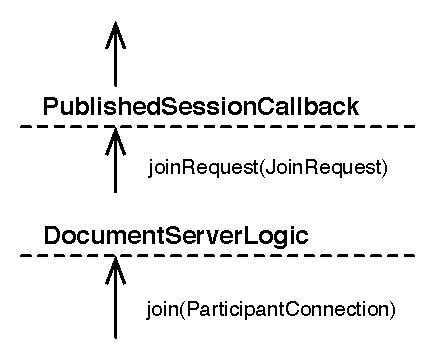
\includegraphics[width=6.88cm,height=5.50cm]{../images/finalreport/architecture_flows/join_request.eps}
 \caption{Publisher receives a JoinRequest}
 \label{fig:archoverview.flow.joinrequest}
\end{figure}

When the request is received from the network layer, the method
\texttt{join} is called on the \texttt{Document\-Server\-Logic} corresponding
to the document the user wants to join. The parameter of type 
\texttt{Participant\-Connection} is used later to communicate with the user
once the join request has been accepted.

The collaboration layer then invokes the \texttt{join\-Request} method on
the \texttt{Published\-Session\-Callback} passing in a \texttt{Join\-Request}
object. The publisher can then either accept or 
reject the request. In the following section, we have a look at the
situation where the publisher accepts the request (rejecting a join
request is even simpler).

\subsubsection{Accepting Join Request}
Now, let us say that the publisher decides
to accept the join request. This happens by calling \texttt{accept} on the
\texttt{Join\-Request} object.

\begin{figure}[H]
 \centering
 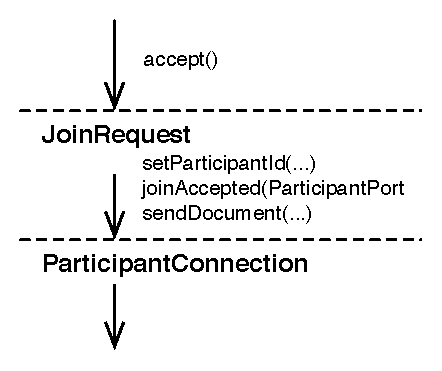
\includegraphics[width=6.91cm,height=5.72cm]{../images/finalreport/architecture_flows/join_request_accept.eps}
 \caption{Publisher accepts the join request}
 \label{fig:archoverview.flow.joinrequestaccept}
\end{figure}

The collaboration layer then invokes the following methods in succession:
\begin{enumerate}
 \item \texttt{setParticipantId} - assigns the participant id
 \item \texttt{joinAccepted} - passes the \texttt{ParticipantPort} to the connection
 \item \texttt{sendDocument} - sends the initial document
\end{enumerate}

The \texttt{Participant\-Port} is used later by the network service to
pass requests from that particular participant (the one that just joined)
to the collaboration layer.

\subsubsection{Join Callback}
\label{sect:archoverview.flow.joinresponse}
The message that the join has been accepted is sent to the joining user. There,
the methods depicted in figure \ref{fig:archoverview.flow.joinresponse}
are called.

\begin{figure}[H]
 \centering
 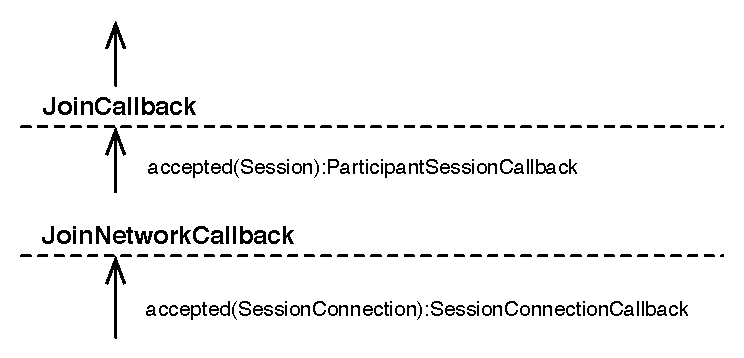
\includegraphics[width=12.03cm,height=5.50cm]{../images/finalreport/architecture_flows/join_response.eps}
 \caption{Joining user receives session}
 \label{fig:archoverview.flow.joinresponse}
\end{figure}

In section \ref{sect:archoverview.flow.initiatejoin} an object of type
\texttt{Join\-Callback} has been passed to the collaboration layer, which in
turn has passed an object of type \texttt{Join\-Network\-Callback} to the
network layer. These callback objects are now used to return the response
of the join.

First, the \texttt{accepted} method is called on the 
\texttt{Join\-Network\-Callback} passing in a \texttt{Session\-Connection},
which is used by the collaboration layer to send messages 
to the session. The \texttt{accepted} method returns an object of type
\texttt{Session\-Connection\-Callback}, which is used by the network layer to
pass received messages from the session to the collaboration layer.

The collaboration layer gives the \texttt{accepted} message to the
\texttt{Join\-Callback} passing along an object of type \texttt{Session}. That
object is used by the application layer to send messages to the session. The
\texttt{Join\-Callback} returns a \texttt{Participant\-Session\-Callback}, which
is used by the collaboration layer to pass received requests to the 
application layer.


\subsection{Communication in the Session}
The figure \ref{fig:archoverview.flow.session} shows how the messages flow
through the layers. The interface between the network and the collaboration
layer as depicted in the figure is only accurate for a participant. The
situation for a publisher is a bit different. The publisher gets a
session (more precisely a \texttt{Published\-Session}) through the
\texttt{publish} method of the \texttt{Collaboration\-Service}. In ACE, both
the publisher and the server part of the session reside on the same
computer. Thus, there is no need for a \texttt{Session\-Connection}. How the
connection between the publisher and the server part is achieved is completely
implementation specific and can thus not be described here.

\begin{figure}[H]
 \centering
 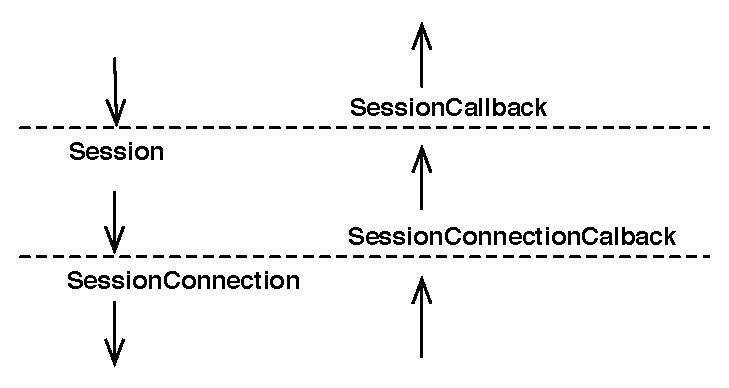
\includegraphics[width=11.78cm,height=6.00cm]{../images/finalreport/architecture_flows/session.eps}
 \caption{Communication in the Session}
 \label{fig:archoverview.flow.session}
\end{figure}


\subsection{Server-Side Communication with Participants}
In the last section we have shown how everything fits together for 
communicating with a session used on the participant side. 
On the side of the publisher (or more specifically
on the host where the published document is hosted) the picture looks 
a bit different. The figure \ref{fig:archoverview.flow.portconnection}
shows the situation on the server.

\begin{figure}[H]
 \centering
 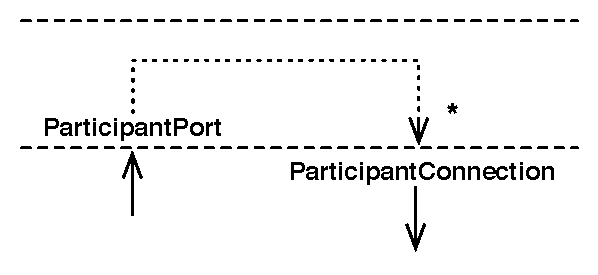
\includegraphics[width=9.56cm,height=4.09cm]{../images/finalreport/architecture_flows/portconnection.eps}
 \caption{Server-side Communication}
 \label{fig:archoverview.flow.portconnection}
\end{figure}

The \texttt{Participant\-Connection} is used by the server-side to communicate
with a particular participant. There is such a connection for each
participant in the session. In the other direction, that is from the
network layer to the collaboration layer, there is a 
\texttt{Participant\-Port} for each participant. The server logic is
responsible to forward messages from one participant (received over the
\texttt{Participant\-Port}) to all other participants (sending over the
\texttt{Participant\-Connection} objects). In between happens the transformation
of requests.

Compare this with the concept of n-way communication introduced in the
introduction chapter about the algorithm 
(see section \ref{sect:algorithm.jupiter.nway}). The 
\texttt{Participant\-Port} and \texttt{Participant\-Connection} represent the
incoming, respectively the outgoing connection of the server-side.


\subsection{Invitations}
When inviting a user into a session, the following steps take place:
\begin{enumerate}
 \item send an invitation to a user (inviter)
 \item receive an invitation (invited user)
 \item accept/reject invitation (invited user)
 \item invitation response at the server 
 \item response to join callback (invited user)
\end{enumerate}

\subsubsection{Sending an Invitation}
The publisher of a document can invite other users to an editing session.
The \texttt{Published\-Session} has a \texttt{invite} method, which serves
exactly that purpose.

\begin{figure}[H]
 \centering
 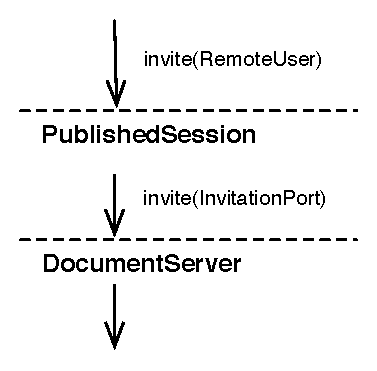
\includegraphics[width=5.82cm,height=5.72cm]{../images/finalreport/architecture_flows/invite_initiate.eps}
 \caption{Invite a user to a session}
 \label{fig:archoverview.flow.inviteinitiate}
\end{figure}

The collaboration layer passes the call to the \texttt{invite} method down
to the \texttt{Document\-Server}. The parameter is of type 
\texttt{Invitation\-Port}, which serves as a callback to the collaboration layer
once the response to the invitation is received.

\subsubsection{Receiving Invitations}
The application layer can register an \texttt{Invitation\-Callback} with
the \texttt{Collaboration\-Service} (\texttt{set\-Invitation\-Callback} method).
This callback object is notified about received invitations.

\begin{figure}[H]
 \centering
 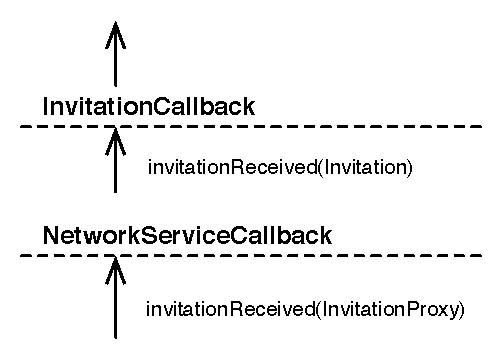
\includegraphics[width=8.96cm,height=5.50cm]{../images/finalreport/architecture_flows/invite_receive.eps}
 \caption{Receiving an invitation}
 \label{fig:archoverview.flow.invitereceive}
\end{figure}

An invitation from another user is passed to the \texttt{invitation\-Received}
method of the \texttt{Network\-Service\-Callback} represented by a
\texttt{Invitation\-Proxy} object. This invitation is passed to the
\texttt{Invitation\-Callback}. 
The \texttt{Invitation\-Callback} has a single method 
\texttt{invitation\-Received} with a parameter of type \texttt{Invitation}.
The \texttt{Invitation} object provides methods to accept or reject
an invitation.

\subsubsection{Accepting an Invitation}
Once the application layer has received an \texttt{Invitation} object, the
invitation can be accepted (and rejected). We have a look now at the situation
where the invitation is accepted.

\begin{figure}[H]
 \centering
 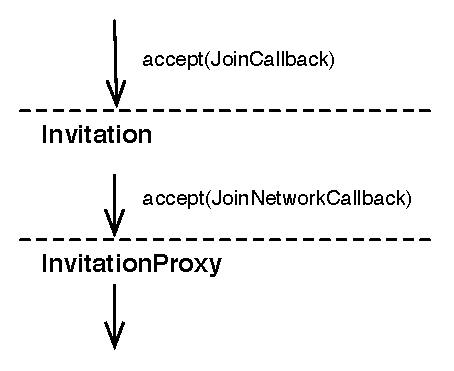
\includegraphics[width=7.13cm,height=5.72cm]{../images/finalreport/architecture_flows/invite_accept.eps}
 \caption{Accepting an inviation}
 \label{fig:archoverview.flow.inviteaccept}
\end{figure}

The \texttt{accept} method takes a \texttt{Join\-Callback} as parameter. The
collaboration layer calls \texttt{accept} on the \texttt{Invitation\-Proxy}
in turn, passing in a \texttt{Join\-Network\-Callback} instance. This is
exactly the same as a join request on a \texttt{Remote\-Document} (see
section \ref{sect:archoverview.flow.initiatejoin}). The session for the
document will be passed to the join callbacks (see section 
\ref{sect:archoverview.flow.joinresponse}).

\subsubsection{Invitation Response on the Server}
Once an invitation has been accepted or rejected by the invited user, a
message is sent back to the publisher. There, the \texttt{Invitation\-Port}
is used to report the server logic about the response.

\begin{figure}[H]
 \centering
 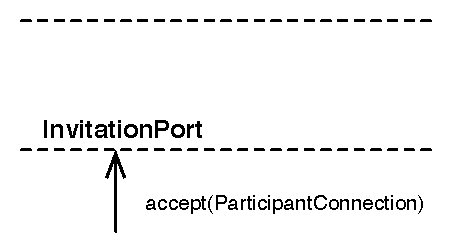
\includegraphics[width=7.16cm,height=3.70cm]{../images/finalreport/architecture_flows/invite_response.eps}
 \caption{Response to invitation on the server}
 \label{fig:archoverview.flow.inviteresponse}
\end{figure}

If the invitation is accepted by the invited user, the \texttt{InvitationPort}'s 
\texttt{accept} method is called passing in a \texttt{ParticipantConnection}.
This \texttt{accept} method is similar to the \texttt{join} method
of the \texttt{DocumentServerLogic}. The only difference is, that an
\texttt{accept} on an \texttt{InvitationPort} lets the invited user into
the session immediately (unless the session has been shutdown in the meantime
in which case the join request is rejected).

The result of the invitation (i.e. rejected or accepted) is not passed to the 
publisher's application layer. 
Future versions of the API might introduce a way to notify the publisher about
accepted/rejected invitations.


\subsection{Explicit User Discovery}
Depending on the employed discovery mechanism by the network layer, the
automatic discovery works only on the local area network. To facilitate
collaboration with other users on the Internet, an explicit user discovery
mechanism exists. 

\subsubsection{Initiating Explicit User Discovery}
\begin{figure}[H]
 \centering
 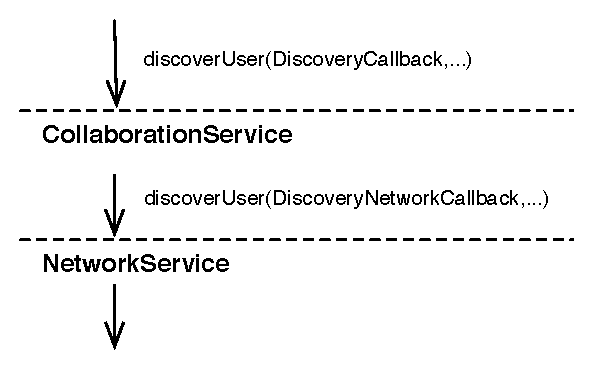
\includegraphics[width=9.49cm,height=5.72cm]{../images/finalreport/architecture_flows/explicitdiscovery.eps}
 \caption{Initiating an explicit user discovery}
 \label{fig:archoverview.flow.explicitdiscovery}
\end{figure}

A \texttt{Discovery\-Callback} as well as an \texttt{Inet\-Address}/port pair 
is passed to the \texttt{Collaboration\-Service}. This request is forwarded
to the \texttt{Network\-Service}.

\subsubsection{Discovery Result}
The result of the explicit user discovery is passed through two different
channels. First, the result (success/failure) is passed to the
\texttt{Discovery\-Callback} (\texttt{Discovery\-Network\-Callback}
respectively).

\begin{figure}[H]
 \centering
 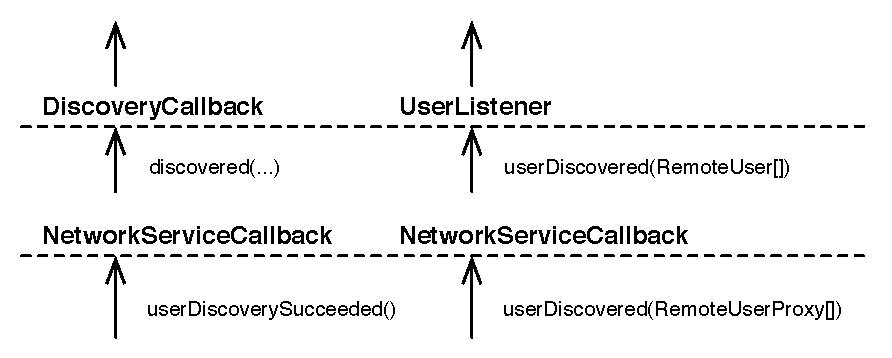
\includegraphics[width=14.53cm,height=5.50cm]{../images/finalreport/architecture_flows/explicitdiscovery_response.eps}
 \caption{The response of explicit user discovery}
 \label{fig:archoverview.flow.explicitdiscoveryresponse}
\end{figure}

If the discovery succeeds, the discovered user is passed through the
\texttt{User\-Listener}s to the application layer (see the section
\ref{sect:archoverview.flow.discovery}).



\section{Reference}
In this section we show which layer is responsible to implement a given
interface.

\subsection{Application Layer}
\begin{itemize}
 \item \texttt{ch.iserver.ace.collaboration.DiscoveryCallback}
 \item \texttt{ch.iserver.ace.collaboration.DocumentListener}
 \item \texttt{ch.iserver.ace.collaboration.InvitationCallback}
 \item \texttt{ch.iserver.ace.collaboration.JoinCallback}
 \item \texttt{ch.iserver.ace.collaboration.ParticipantSessionCallback}
 \item \texttt{ch.iserver.ace.collaboration.PublishedSessionCallback}
 \item \texttt{ch.iserver.ace.collaboration.ServiceFailureHandler}
 \item \texttt{ch.iserver.ace.collaboration.SessionCallback}
 \item \texttt{ch.iserver.ace.collaboration.UserListener}
\end{itemize}

\subsection{Collaboration Layer}
\begin{itemize}
 \item \texttt{ch.iserver.ace.collaboration.CollaborationService}
 \item \texttt{ch.iserver.ace.collaboration.Invitation}
 \item \texttt{ch.iserver.ace.collaboration.JoinRequest}
 \item \texttt{ch.iserver.ace.collaboration.Participant}
 \item \texttt{ch.iserver.ace.collaboration.PortableDocument}
 \item \texttt{ch.iserver.ace.collaboration.PublishedSession}
 \item \texttt{ch.iserver.ace.collaboration.RemoteDocument}
 \item \texttt{ch.iserver.ace.collaboration.RemoteUser}
 \item \texttt{ch.iserver.ace.collaboration.Session}
 \item \texttt{ch.iserver.ace.net.DiscoveryNetworkCallback}
 \item \texttt{ch.iserver.ace.net.DocumentServerLogic}
 \item \texttt{ch.iserver.ace.net.InvitationPort}
 \item \texttt{ch.iserver.ace.net.JoinNetworkCallback}
 \item \texttt{ch.iserver.ace.net.NetworkServiceCallback}
 \item \texttt{ch.iserver.ace.net.ParticipantPort}
 \item \texttt{ch.iserver.ace.net.SessionConnectionCallback}  
\end{itemize}

\subsection{Network Layer}
\begin{itemize}
 \item \texttt{ch.iserver.ace.net.DocumentServer}
 \item \texttt{ch.iserver.ace.net.InvitationProxy}
 \item \texttt{ch.iserver.ace.net.NetworkService}
 \item \texttt{ch.iserver.ace.net.ParticipantConnection}
 \item \texttt{ch.iserver.ace.net.PortableDocument}
 \item \texttt{ch.iserver.ace.net.RemoteDocumentProxy}
 \item \texttt{ch.iserver.ace.net.RemoteUserProxy}
 \item \texttt{ch.iserver.ace.net.SessionConnection}     
\end{itemize}
